% Created by tikzDevice version 0.12.4 on 2023-10-09 16:01:45
% !TEX encoding = UTF-8 Unicode
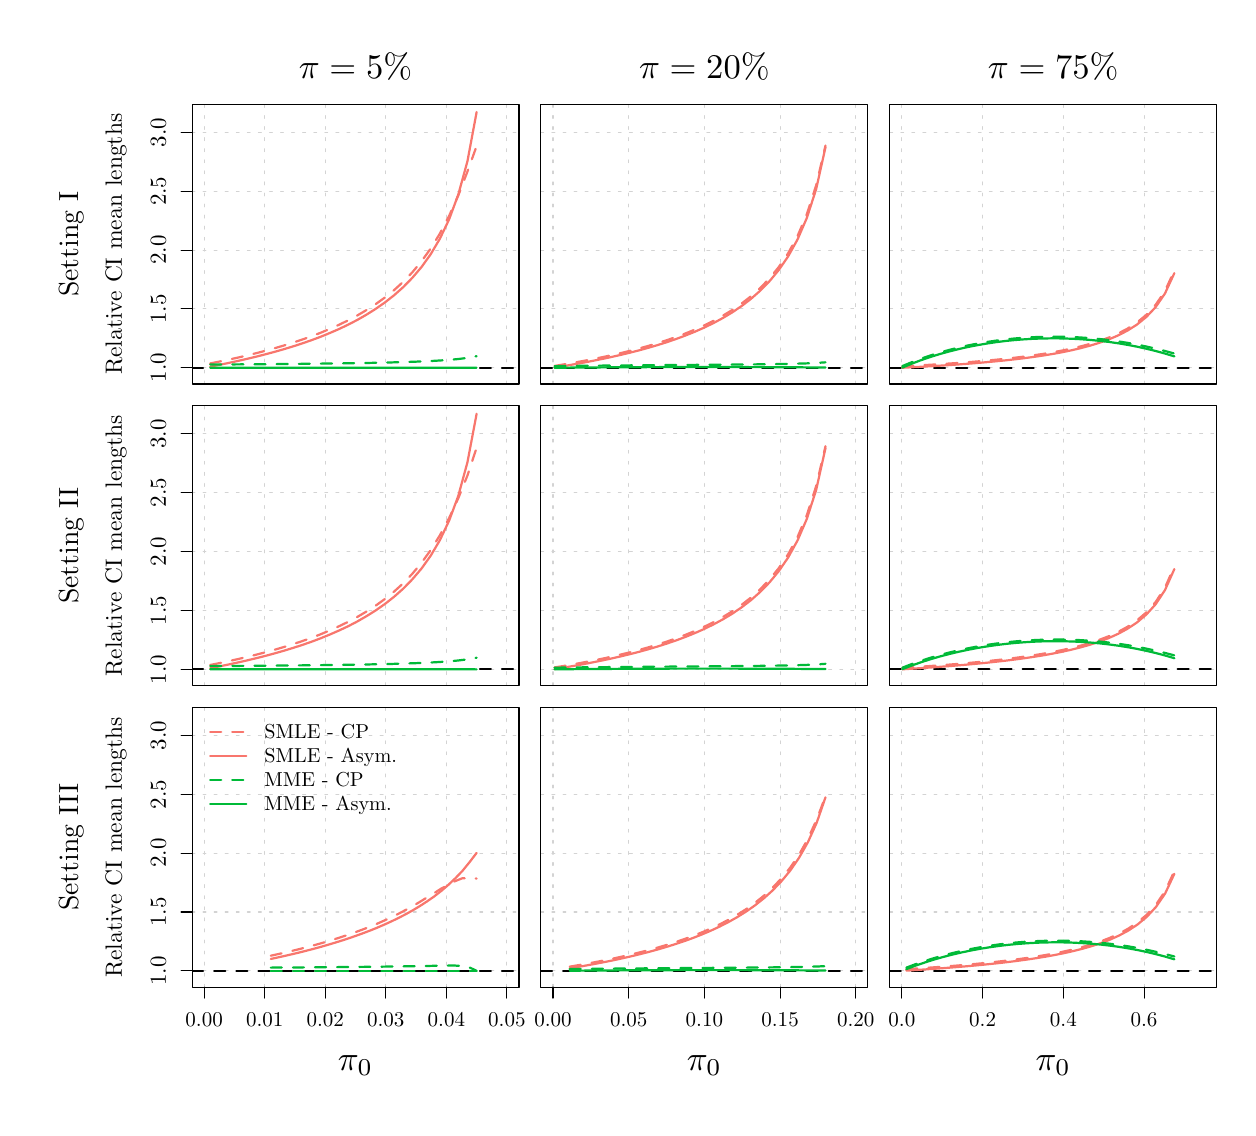
\begin{tikzpicture}[x=1pt,y=1pt]
\definecolor{fillColor}{RGB}{255,255,255}
\path[use as bounding box,fill=fillColor,fill opacity=0.00] (0,0) rectangle (433.62,390.26);
\begin{scope}
\path[clip] ( 55.44,257.53) rectangle (181.50,366.50);
\definecolor{drawColor}{RGB}{0,0,0}

\node[text=drawColor,anchor=base,inner sep=0pt, outer sep=0pt, scale=  0.66] at (118.47,231.40) {Simulation ID};

\node[text=drawColor,rotate= 90.00,anchor=base,inner sep=0pt, outer sep=0pt, scale=  0.66] at ( 34.06,312.01) {Ratio of RMSE};
\end{scope}
\begin{scope}
\path[clip] (  0.00,  0.00) rectangle (433.62,390.26);
\definecolor{drawColor}{RGB}{0,0,0}

\path[draw=drawColor,line width= 0.4pt,line join=round,line cap=round] ( 59.40,267.36) -- ( 59.40,352.42);

\path[draw=drawColor,line width= 0.4pt,line join=round,line cap=round] ( 59.40,267.36) -- ( 55.44,267.36);

\path[draw=drawColor,line width= 0.4pt,line join=round,line cap=round] ( 59.40,288.62) -- ( 55.44,288.62);

\path[draw=drawColor,line width= 0.4pt,line join=round,line cap=round] ( 59.40,309.89) -- ( 55.44,309.89);

\path[draw=drawColor,line width= 0.4pt,line join=round,line cap=round] ( 59.40,331.15) -- ( 55.44,331.15);

\path[draw=drawColor,line width= 0.4pt,line join=round,line cap=round] ( 59.40,352.42) -- ( 55.44,352.42);

\node[text=drawColor,rotate= 90.00,anchor=base,inner sep=0pt, outer sep=0pt, scale=  0.83] at ( 49.90,267.36) {1.0};

\node[text=drawColor,rotate= 90.00,anchor=base,inner sep=0pt, outer sep=0pt, scale=  0.83] at ( 49.90,288.62) {1.5};

\node[text=drawColor,rotate= 90.00,anchor=base,inner sep=0pt, outer sep=0pt, scale=  0.83] at ( 49.90,309.89) {2.0};

\node[text=drawColor,rotate= 90.00,anchor=base,inner sep=0pt, outer sep=0pt, scale=  0.83] at ( 49.90,331.15) {2.5};

\node[text=drawColor,rotate= 90.00,anchor=base,inner sep=0pt, outer sep=0pt, scale=  0.83] at ( 49.90,352.42) {3.0};
\end{scope}
\begin{scope}
\path[clip] ( 59.40,261.49) rectangle (177.54,362.54);
\definecolor{drawColor}{RGB}{211,211,211}

\path[draw=drawColor,line width= 0.4pt,dash pattern=on 1pt off 3pt ,line join=round,line cap=round] ( 63.78,261.49) -- ( 63.78,362.54);

\path[draw=drawColor,line width= 0.4pt,dash pattern=on 1pt off 3pt ,line join=round,line cap=round] ( 85.65,261.49) -- ( 85.65,362.54);

\path[draw=drawColor,line width= 0.4pt,dash pattern=on 1pt off 3pt ,line join=round,line cap=round] (107.53,261.49) -- (107.53,362.54);

\path[draw=drawColor,line width= 0.4pt,dash pattern=on 1pt off 3pt ,line join=round,line cap=round] (129.41,261.49) -- (129.41,362.54);

\path[draw=drawColor,line width= 0.4pt,dash pattern=on 1pt off 3pt ,line join=round,line cap=round] (151.29,261.49) -- (151.29,362.54);

\path[draw=drawColor,line width= 0.4pt,dash pattern=on 1pt off 3pt ,line join=round,line cap=round] (173.16,261.49) -- (173.16,362.54);

\path[draw=drawColor,line width= 0.4pt,dash pattern=on 1pt off 3pt ,line join=round,line cap=round] ( 59.40,267.36) -- (177.54,267.36);

\path[draw=drawColor,line width= 0.4pt,dash pattern=on 1pt off 3pt ,line join=round,line cap=round] ( 59.40,288.62) -- (177.54,288.62);

\path[draw=drawColor,line width= 0.4pt,dash pattern=on 1pt off 3pt ,line join=round,line cap=round] ( 59.40,309.89) -- (177.54,309.89);

\path[draw=drawColor,line width= 0.4pt,dash pattern=on 1pt off 3pt ,line join=round,line cap=round] ( 59.40,331.15) -- (177.54,331.15);

\path[draw=drawColor,line width= 0.4pt,dash pattern=on 1pt off 3pt ,line join=round,line cap=round] ( 59.40,352.42) -- (177.54,352.42);
\end{scope}
\begin{scope}
\path[clip] (  0.00,  0.00) rectangle (433.62,390.26);
\definecolor{drawColor}{RGB}{0,0,0}

\path[draw=drawColor,line width= 0.4pt,line join=round,line cap=round] ( 59.40,261.49) --
	(177.54,261.49) --
	(177.54,362.54) --
	( 59.40,362.54) --
	cycle;
\end{scope}
\begin{scope}
\path[clip] ( 59.40,261.49) rectangle (177.54,362.54);
\definecolor{drawColor}{RGB}{0,0,0}

\path[draw=drawColor,line width= 0.8pt,dash pattern=on 4pt off 4pt ,line join=round,line cap=round] ( 59.40,267.36) -- (177.54,267.36);
\definecolor{drawColor}{RGB}{248,118,109}

\path[draw=drawColor,line width= 0.8pt,dash pattern=on 4pt off 4pt ,line join=round,line cap=round] ( 65.96,268.93) --
	( 69.28,269.60) --
	( 72.60,270.30) --
	( 75.92,271.03) --
	( 79.24,271.81) --
	( 82.56,272.63) --
	( 85.88,273.49) --
	( 89.20,274.41) --
	( 92.52,275.39) --
	( 95.84,276.43) --
	( 99.16,277.53) --
	(102.48,278.72) --
	(105.80,279.99) --
	(109.12,281.38) --
	(112.43,282.86) --
	(115.75,284.47) --
	(119.07,286.24) --
	(122.39,288.19) --
	(125.71,290.33) --
	(129.03,292.71) --
	(132.35,295.37) --
	(135.67,298.40) --
	(138.99,301.86) --
	(142.31,305.84) --
	(145.63,310.45) --
	(148.95,315.85) --
	(152.27,322.23) --
	(155.59,329.60) --
	(158.91,338.26) --
	(162.23,347.50);

\path[draw=drawColor,line width= 0.8pt,line join=round,line cap=round] ( 65.96,267.77) --
	( 69.28,268.42) --
	( 72.60,269.10) --
	( 75.92,269.82) --
	( 79.24,270.58) --
	( 82.56,271.37) --
	( 85.88,272.22) --
	( 89.20,273.11) --
	( 92.52,274.06) --
	( 95.84,275.07) --
	( 99.16,276.15) --
	(102.48,277.30) --
	(105.80,278.54) --
	(109.12,279.90) --
	(112.43,281.33) --
	(115.75,282.91) --
	(119.07,284.63) --
	(122.39,286.53) --
	(125.71,288.61) --
	(129.03,290.93) --
	(132.35,293.52) --
	(135.67,296.47) --
	(138.99,299.86) --
	(142.31,303.76) --
	(145.63,308.39) --
	(148.95,314.00) --
	(152.27,320.95) --
	(155.59,329.91) --
	(158.91,342.00) --
	(162.23,359.78);
\definecolor{drawColor}{RGB}{0,186,56}

\path[draw=drawColor,line width= 0.8pt,line join=round,line cap=round] ( 65.96,267.36) --
	( 69.28,267.36) --
	( 72.60,267.36) --
	( 75.92,267.37) --
	( 79.24,267.37) --
	( 82.56,267.37) --
	( 85.88,267.37) --
	( 89.20,267.37) --
	( 92.52,267.37) --
	( 95.84,267.37) --
	( 99.16,267.37) --
	(102.48,267.37) --
	(105.80,267.37) --
	(109.12,267.37) --
	(112.43,267.37) --
	(115.75,267.37) --
	(119.07,267.37) --
	(122.39,267.37) --
	(125.71,267.37) --
	(129.03,267.37) --
	(132.35,267.37) --
	(135.67,267.37) --
	(138.99,267.37) --
	(142.31,267.37) --
	(145.63,267.38) --
	(148.95,267.38) --
	(152.27,267.38) --
	(155.59,267.37) --
	(158.91,267.38) --
	(162.23,267.37);

\path[draw=drawColor,line width= 0.8pt,dash pattern=on 4pt off 4pt ,line join=round,line cap=round] ( 65.96,268.52) --
	( 69.28,268.54) --
	( 72.60,268.56) --
	( 75.92,268.59) --
	( 79.24,268.61) --
	( 82.56,268.63) --
	( 85.88,268.66) --
	( 89.20,268.69) --
	( 92.52,268.72) --
	( 95.84,268.75) --
	( 99.16,268.78) --
	(102.48,268.82) --
	(105.80,268.86) --
	(109.12,268.90) --
	(112.43,268.94) --
	(115.75,268.99) --
	(119.07,269.04) --
	(122.39,269.10) --
	(125.71,269.16) --
	(129.03,269.24) --
	(132.35,269.32) --
	(135.67,269.42) --
	(138.99,269.52) --
	(142.31,269.65) --
	(145.63,269.80) --
	(148.95,269.99) --
	(152.27,270.22) --
	(155.59,270.52) --
	(158.91,270.93) --
	(162.23,271.54);
\end{scope}
\begin{scope}
\path[clip] (  0.00,  0.00) rectangle (433.62,390.26);
\definecolor{drawColor}{RGB}{0,0,0}

\node[text=drawColor,rotate= 90.00,anchor=base,inner sep=0pt, outer sep=0pt, scale=  1.00] at ( 18.22,312.01) {Setting I};

\node[text=drawColor,rotate= 90.00,anchor=base,inner sep=0pt, outer sep=0pt, scale=  0.85] at ( 34.06,312.01) {Relative CI mean lengths};

\node[text=drawColor,anchor=base,inner sep=0pt, outer sep=0pt, scale=  1.25] at (118.47,372.04) {$\pi = 5\%$};
\end{scope}
\begin{scope}
\path[clip] (181.50,257.53) rectangle (307.56,366.50);
\definecolor{drawColor}{RGB}{0,0,0}

\node[text=drawColor,anchor=base,inner sep=0pt, outer sep=0pt, scale=  0.66] at (244.53,231.40) {Simulation ID};

\node[text=drawColor,rotate= 90.00,anchor=base,inner sep=0pt, outer sep=0pt, scale=  0.66] at (160.12,312.01) {Ratio of RMSE};
\end{scope}
\begin{scope}
\path[clip] (185.46,261.49) rectangle (303.60,362.54);
\definecolor{drawColor}{RGB}{211,211,211}

\path[draw=drawColor,line width= 0.4pt,dash pattern=on 1pt off 3pt ,line join=round,line cap=round] (189.84,261.49) -- (189.84,362.54);

\path[draw=drawColor,line width= 0.4pt,dash pattern=on 1pt off 3pt ,line join=round,line cap=round] (217.18,261.49) -- (217.18,362.54);

\path[draw=drawColor,line width= 0.4pt,dash pattern=on 1pt off 3pt ,line join=round,line cap=round] (244.53,261.49) -- (244.53,362.54);

\path[draw=drawColor,line width= 0.4pt,dash pattern=on 1pt off 3pt ,line join=round,line cap=round] (271.88,261.49) -- (271.88,362.54);

\path[draw=drawColor,line width= 0.4pt,dash pattern=on 1pt off 3pt ,line join=round,line cap=round] (299.22,261.49) -- (299.22,362.54);

\path[draw=drawColor,line width= 0.4pt,dash pattern=on 1pt off 3pt ,line join=round,line cap=round] (185.46,267.36) -- (303.60,267.36);

\path[draw=drawColor,line width= 0.4pt,dash pattern=on 1pt off 3pt ,line join=round,line cap=round] (185.46,288.62) -- (303.60,288.62);

\path[draw=drawColor,line width= 0.4pt,dash pattern=on 1pt off 3pt ,line join=round,line cap=round] (185.46,309.89) -- (303.60,309.89);

\path[draw=drawColor,line width= 0.4pt,dash pattern=on 1pt off 3pt ,line join=round,line cap=round] (185.46,331.15) -- (303.60,331.15);

\path[draw=drawColor,line width= 0.4pt,dash pattern=on 1pt off 3pt ,line join=round,line cap=round] (185.46,352.42) -- (303.60,352.42);
\end{scope}
\begin{scope}
\path[clip] (  0.00,  0.00) rectangle (433.62,390.26);
\definecolor{drawColor}{RGB}{0,0,0}

\path[draw=drawColor,line width= 0.4pt,line join=round,line cap=round] (185.46,261.49) --
	(303.60,261.49) --
	(303.60,362.54) --
	(185.46,362.54) --
	cycle;
\end{scope}
\begin{scope}
\path[clip] (185.46,261.49) rectangle (303.60,362.54);
\definecolor{drawColor}{RGB}{0,0,0}

\path[draw=drawColor,line width= 0.8pt,dash pattern=on 4pt off 4pt ,line join=round,line cap=round] (185.46,267.36) -- (303.60,267.36);
\definecolor{drawColor}{RGB}{248,118,109}

\path[draw=drawColor,line width= 0.8pt,dash pattern=on 4pt off 4pt ,line join=round,line cap=round] (190.38,268.03) --
	(193.76,268.59) --
	(197.13,269.17) --
	(200.51,269.78) --
	(203.89,270.42) --
	(207.26,271.11) --
	(210.64,271.83) --
	(214.01,272.60) --
	(217.39,273.42) --
	(220.77,274.29) --
	(224.14,275.23) --
	(227.52,276.23) --
	(230.89,277.31) --
	(234.27,278.48) --
	(237.65,279.75) --
	(241.02,281.13) --
	(244.40,282.64) --
	(247.77,284.30) --
	(251.15,286.15) --
	(254.53,288.20) --
	(257.90,290.51) --
	(261.28,293.13) --
	(264.65,296.13) --
	(268.03,299.63) --
	(271.41,303.77) --
	(274.78,308.73) --
	(278.16,314.90) --
	(281.53,322.79) --
	(284.91,333.26) --
	(288.29,347.66);

\path[draw=drawColor,line width= 0.8pt,line join=round,line cap=round] (190.38,267.45) --
	(193.76,267.99) --
	(197.13,268.56) --
	(200.51,269.16) --
	(203.89,269.80) --
	(207.26,270.47) --
	(210.64,271.19) --
	(214.01,271.95) --
	(217.39,272.75) --
	(220.77,273.62) --
	(224.14,274.54) --
	(227.52,275.53) --
	(230.89,276.59) --
	(234.27,277.75) --
	(237.65,279.00) --
	(241.02,280.36) --
	(244.40,281.85) --
	(247.77,283.49) --
	(251.15,285.31) --
	(254.53,287.34) --
	(257.90,289.61) --
	(261.28,292.20) --
	(264.65,295.16) --
	(268.03,298.61) --
	(271.41,302.69) --
	(274.78,307.59) --
	(278.16,313.68) --
	(281.53,321.46) --
	(284.91,331.89) --
	(288.29,347.07);
\definecolor{drawColor}{RGB}{0,186,56}

\path[draw=drawColor,line width= 0.8pt,line join=round,line cap=round] (190.38,267.37) --
	(193.76,267.40) --
	(197.13,267.43) --
	(200.51,267.45) --
	(203.89,267.48) --
	(207.26,267.50) --
	(210.64,267.52) --
	(214.01,267.54) --
	(217.39,267.56) --
	(220.77,267.58) --
	(224.14,267.59) --
	(227.52,267.60) --
	(230.89,267.61) --
	(234.27,267.62) --
	(237.65,267.62) --
	(241.02,267.62) --
	(244.40,267.63) --
	(247.77,267.63) --
	(251.15,267.62) --
	(254.53,267.62) --
	(257.90,267.61) --
	(261.28,267.60) --
	(264.65,267.59) --
	(268.03,267.58) --
	(271.41,267.56) --
	(274.78,267.55) --
	(278.16,267.53) --
	(281.53,267.50) --
	(284.91,267.48) --
	(288.29,267.46);

\path[draw=drawColor,line width= 0.8pt,dash pattern=on 4pt off 4pt ,line join=round,line cap=round] (190.38,267.95) --
	(193.76,267.99) --
	(197.13,268.03) --
	(200.51,268.07) --
	(203.89,268.10) --
	(207.26,268.14) --
	(210.64,268.17) --
	(214.01,268.20) --
	(217.39,268.23) --
	(220.77,268.26) --
	(224.14,268.29) --
	(227.52,268.31) --
	(230.89,268.34) --
	(234.27,268.36) --
	(237.65,268.39) --
	(241.02,268.41) --
	(244.40,268.44) --
	(247.77,268.46) --
	(251.15,268.49) --
	(254.53,268.51) --
	(257.90,268.54) --
	(261.28,268.57) --
	(264.65,268.61) --
	(268.03,268.65) --
	(271.41,268.70) --
	(274.78,268.77) --
	(278.16,268.85) --
	(281.53,268.95) --
	(284.91,269.10) --
	(288.29,269.33);
\end{scope}
\begin{scope}
\path[clip] (  0.00,  0.00) rectangle (433.62,390.26);
\definecolor{drawColor}{RGB}{0,0,0}

\node[text=drawColor,anchor=base,inner sep=0pt, outer sep=0pt, scale=  1.25] at (244.53,372.04) {$\pi = 20\%$};
\end{scope}
\begin{scope}
\path[clip] (307.56,257.53) rectangle (433.62,366.50);
\definecolor{drawColor}{RGB}{0,0,0}

\node[text=drawColor,anchor=base,inner sep=0pt, outer sep=0pt, scale=  0.66] at (370.59,231.40) {Simulation ID};

\node[text=drawColor,rotate= 90.00,anchor=base,inner sep=0pt, outer sep=0pt, scale=  0.66] at (286.18,312.01) {Ratio of RMSE};
\end{scope}
\begin{scope}
\path[clip] (311.52,261.49) rectangle (429.66,362.54);
\definecolor{drawColor}{RGB}{211,211,211}

\path[draw=drawColor,line width= 0.4pt,dash pattern=on 1pt off 3pt ,line join=round,line cap=round] (315.90,261.49) -- (315.90,362.54);

\path[draw=drawColor,line width= 0.4pt,dash pattern=on 1pt off 3pt ,line join=round,line cap=round] (345.07,261.49) -- (345.07,362.54);

\path[draw=drawColor,line width= 0.4pt,dash pattern=on 1pt off 3pt ,line join=round,line cap=round] (374.24,261.49) -- (374.24,362.54);

\path[draw=drawColor,line width= 0.4pt,dash pattern=on 1pt off 3pt ,line join=round,line cap=round] (403.41,261.49) -- (403.41,362.54);

\path[draw=drawColor,line width= 0.4pt,dash pattern=on 1pt off 3pt ,line join=round,line cap=round] (311.52,267.36) -- (429.66,267.36);

\path[draw=drawColor,line width= 0.4pt,dash pattern=on 1pt off 3pt ,line join=round,line cap=round] (311.52,288.62) -- (429.66,288.62);

\path[draw=drawColor,line width= 0.4pt,dash pattern=on 1pt off 3pt ,line join=round,line cap=round] (311.52,309.89) -- (429.66,309.89);

\path[draw=drawColor,line width= 0.4pt,dash pattern=on 1pt off 3pt ,line join=round,line cap=round] (311.52,331.15) -- (429.66,331.15);

\path[draw=drawColor,line width= 0.4pt,dash pattern=on 1pt off 3pt ,line join=round,line cap=round] (311.52,352.42) -- (429.66,352.42);
\end{scope}
\begin{scope}
\path[clip] (  0.00,  0.00) rectangle (433.62,390.26);
\definecolor{drawColor}{RGB}{0,0,0}

\path[draw=drawColor,line width= 0.4pt,line join=round,line cap=round] (311.52,261.49) --
	(429.66,261.49) --
	(429.66,362.54) --
	(311.52,362.54) --
	cycle;
\end{scope}
\begin{scope}
\path[clip] (311.52,261.49) rectangle (429.66,362.54);
\definecolor{drawColor}{RGB}{0,0,0}

\path[draw=drawColor,line width= 0.8pt,dash pattern=on 4pt off 4pt ,line join=round,line cap=round] (311.52,267.36) -- (429.66,267.36);
\definecolor{drawColor}{RGB}{248,118,109}

\path[draw=drawColor,line width= 0.8pt,dash pattern=on 4pt off 4pt ,line join=round,line cap=round] (316.04,267.91) --
	(319.43,268.08) --
	(322.82,268.26) --
	(326.21,268.46) --
	(329.60,268.66) --
	(332.99,268.89) --
	(336.38,269.12) --
	(339.77,269.38) --
	(343.16,269.65) --
	(346.55,269.95) --
	(349.94,270.27) --
	(353.33,270.62) --
	(356.72,271.00) --
	(360.11,271.41) --
	(363.50,271.87) --
	(366.89,272.37) --
	(370.28,272.93) --
	(373.67,273.56) --
	(377.06,274.27) --
	(380.45,275.07) --
	(383.84,275.98) --
	(387.23,277.04) --
	(390.62,278.26) --
	(394.01,279.73) --
	(397.40,281.50) --
	(400.79,283.68) --
	(404.18,286.45) --
	(407.57,290.08) --
	(410.96,295.09) --
	(414.35,302.52);

\path[draw=drawColor,line width= 0.8pt,line join=round,line cap=round] (316.04,267.37) --
	(319.43,267.54) --
	(322.82,267.72) --
	(326.21,267.91) --
	(329.60,268.12) --
	(332.99,268.33) --
	(336.38,268.57) --
	(339.77,268.82) --
	(343.16,269.09) --
	(346.55,269.39) --
	(349.94,269.70) --
	(353.33,270.04) --
	(356.72,270.42) --
	(360.11,270.83) --
	(363.50,271.28) --
	(366.89,271.78) --
	(370.28,272.33) --
	(373.67,272.95) --
	(377.06,273.65) --
	(380.45,274.44) --
	(383.84,275.34) --
	(387.23,276.38) --
	(390.62,277.59) --
	(394.01,279.04) --
	(397.40,280.79) --
	(400.79,282.94) --
	(404.18,285.68) --
	(407.57,289.26) --
	(410.96,294.21) --
	(414.35,301.55);
\definecolor{drawColor}{RGB}{0,186,56}

\path[draw=drawColor,line width= 0.8pt,line join=round,line cap=round] (316.04,267.42) --
	(319.43,268.83) --
	(322.82,270.11) --
	(326.21,271.27) --
	(329.60,272.32) --
	(332.99,273.26) --
	(336.38,274.11) --
	(339.77,274.87) --
	(343.16,275.53) --
	(346.55,276.11) --
	(349.94,276.62) --
	(353.33,277.04) --
	(356.72,277.38) --
	(360.11,277.64) --
	(363.50,277.84) --
	(366.89,277.95) --
	(370.28,278.00) --
	(373.67,277.97) --
	(377.06,277.86) --
	(380.45,277.69) --
	(383.84,277.43) --
	(387.23,277.10) --
	(390.62,276.71) --
	(394.01,276.22) --
	(397.40,275.65) --
	(400.79,275.00) --
	(404.18,274.26) --
	(407.57,273.43) --
	(410.96,272.50) --
	(414.35,271.48);

\path[draw=drawColor,line width= 0.8pt,dash pattern=on 4pt off 4pt ,line join=round,line cap=round] (316.04,267.96) --
	(319.43,269.37) --
	(322.82,270.65) --
	(326.21,271.81) --
	(329.60,272.86) --
	(332.99,273.81) --
	(336.38,274.66) --
	(339.77,275.42) --
	(343.16,276.09) --
	(346.55,276.67) --
	(349.94,277.17) --
	(353.33,277.60) --
	(356.72,277.95) --
	(360.11,278.22) --
	(363.50,278.42) --
	(366.89,278.54) --
	(370.28,278.59) --
	(373.67,278.57) --
	(377.06,278.48) --
	(380.45,278.31) --
	(383.84,278.07) --
	(387.23,277.76) --
	(390.62,277.38) --
	(394.01,276.91) --
	(397.40,276.37) --
	(400.79,275.75) --
	(404.18,275.05) --
	(407.57,274.27) --
	(410.96,273.42) --
	(414.35,272.50);
\end{scope}
\begin{scope}
\path[clip] (  0.00,  0.00) rectangle (433.62,390.26);
\definecolor{drawColor}{RGB}{0,0,0}

\node[text=drawColor,anchor=base,inner sep=0pt, outer sep=0pt, scale=  1.25] at (370.59,372.04) {$\pi = 75\%$};
\end{scope}
\begin{scope}
\path[clip] ( 55.44,148.57) rectangle (181.50,257.53);
\definecolor{drawColor}{RGB}{0,0,0}

\node[text=drawColor,anchor=base,inner sep=0pt, outer sep=0pt, scale=  0.66] at (118.47,122.43) {Simulation ID};

\node[text=drawColor,rotate= 90.00,anchor=base,inner sep=0pt, outer sep=0pt, scale=  0.66] at ( 34.06,203.05) {Ratio of RMSE};
\end{scope}
\begin{scope}
\path[clip] (  0.00,  0.00) rectangle (433.62,390.26);
\definecolor{drawColor}{RGB}{0,0,0}

\path[draw=drawColor,line width= 0.4pt,line join=round,line cap=round] ( 59.40,158.39) -- ( 59.40,243.45);

\path[draw=drawColor,line width= 0.4pt,line join=round,line cap=round] ( 59.40,158.39) -- ( 55.44,158.39);

\path[draw=drawColor,line width= 0.4pt,line join=round,line cap=round] ( 59.40,179.66) -- ( 55.44,179.66);

\path[draw=drawColor,line width= 0.4pt,line join=round,line cap=round] ( 59.40,200.92) -- ( 55.44,200.92);

\path[draw=drawColor,line width= 0.4pt,line join=round,line cap=round] ( 59.40,222.19) -- ( 55.44,222.19);

\path[draw=drawColor,line width= 0.4pt,line join=round,line cap=round] ( 59.40,243.45) -- ( 55.44,243.45);

\node[text=drawColor,rotate= 90.00,anchor=base,inner sep=0pt, outer sep=0pt, scale=  0.83] at ( 49.90,158.39) {1.0};

\node[text=drawColor,rotate= 90.00,anchor=base,inner sep=0pt, outer sep=0pt, scale=  0.83] at ( 49.90,179.66) {1.5};

\node[text=drawColor,rotate= 90.00,anchor=base,inner sep=0pt, outer sep=0pt, scale=  0.83] at ( 49.90,200.92) {2.0};

\node[text=drawColor,rotate= 90.00,anchor=base,inner sep=0pt, outer sep=0pt, scale=  0.83] at ( 49.90,222.19) {2.5};

\node[text=drawColor,rotate= 90.00,anchor=base,inner sep=0pt, outer sep=0pt, scale=  0.83] at ( 49.90,243.45) {3.0};
\end{scope}
\begin{scope}
\path[clip] ( 59.40,152.53) rectangle (177.54,253.57);
\definecolor{drawColor}{RGB}{211,211,211}

\path[draw=drawColor,line width= 0.4pt,dash pattern=on 1pt off 3pt ,line join=round,line cap=round] ( 63.78,152.53) -- ( 63.78,253.57);

\path[draw=drawColor,line width= 0.4pt,dash pattern=on 1pt off 3pt ,line join=round,line cap=round] ( 85.65,152.53) -- ( 85.65,253.57);

\path[draw=drawColor,line width= 0.4pt,dash pattern=on 1pt off 3pt ,line join=round,line cap=round] (107.53,152.53) -- (107.53,253.57);

\path[draw=drawColor,line width= 0.4pt,dash pattern=on 1pt off 3pt ,line join=round,line cap=round] (129.41,152.53) -- (129.41,253.57);

\path[draw=drawColor,line width= 0.4pt,dash pattern=on 1pt off 3pt ,line join=round,line cap=round] (151.29,152.53) -- (151.29,253.57);

\path[draw=drawColor,line width= 0.4pt,dash pattern=on 1pt off 3pt ,line join=round,line cap=round] (173.16,152.53) -- (173.16,253.57);

\path[draw=drawColor,line width= 0.4pt,dash pattern=on 1pt off 3pt ,line join=round,line cap=round] ( 59.40,158.39) -- (177.54,158.39);

\path[draw=drawColor,line width= 0.4pt,dash pattern=on 1pt off 3pt ,line join=round,line cap=round] ( 59.40,179.66) -- (177.54,179.66);

\path[draw=drawColor,line width= 0.4pt,dash pattern=on 1pt off 3pt ,line join=round,line cap=round] ( 59.40,200.92) -- (177.54,200.92);

\path[draw=drawColor,line width= 0.4pt,dash pattern=on 1pt off 3pt ,line join=round,line cap=round] ( 59.40,222.19) -- (177.54,222.19);

\path[draw=drawColor,line width= 0.4pt,dash pattern=on 1pt off 3pt ,line join=round,line cap=round] ( 59.40,243.45) -- (177.54,243.45);
\end{scope}
\begin{scope}
\path[clip] (  0.00,  0.00) rectangle (433.62,390.26);
\definecolor{drawColor}{RGB}{0,0,0}

\path[draw=drawColor,line width= 0.4pt,line join=round,line cap=round] ( 59.40,152.53) --
	(177.54,152.53) --
	(177.54,253.57) --
	( 59.40,253.57) --
	cycle;
\end{scope}
\begin{scope}
\path[clip] ( 59.40,152.53) rectangle (177.54,253.57);
\definecolor{drawColor}{RGB}{0,0,0}

\path[draw=drawColor,line width= 0.8pt,dash pattern=on 4pt off 4pt ,line join=round,line cap=round] ( 59.40,158.39) -- (177.54,158.39);
\definecolor{drawColor}{RGB}{248,118,109}

\path[draw=drawColor,line width= 0.8pt,dash pattern=on 4pt off 4pt ,line join=round,line cap=round] ( 65.96,159.98) --
	( 69.28,160.64) --
	( 72.60,161.35) --
	( 75.92,162.08) --
	( 79.24,162.86) --
	( 82.56,163.68) --
	( 85.88,164.55) --
	( 89.20,165.46) --
	( 92.52,166.44) --
	( 95.84,167.48) --
	( 99.16,168.58) --
	(102.48,169.76) --
	(105.80,171.04) --
	(109.12,172.44) --
	(112.43,173.93) --
	(115.75,175.53) --
	(119.07,177.30) --
	(122.39,179.26) --
	(125.71,181.38) --
	(129.03,183.77) --
	(132.35,186.44) --
	(135.67,189.46) --
	(138.99,192.92) --
	(142.31,196.89) --
	(145.63,201.48) --
	(148.95,206.83) --
	(152.27,213.03) --
	(155.59,220.19) --
	(158.91,228.43) --
	(162.23,238.46);

\path[draw=drawColor,line width= 0.8pt,line join=round,line cap=round] ( 65.96,158.81) --
	( 69.28,159.46) --
	( 72.60,160.14) --
	( 75.92,160.86) --
	( 79.24,161.61) --
	( 82.56,162.41) --
	( 85.88,163.25) --
	( 89.20,164.15) --
	( 92.52,165.10) --
	( 95.84,166.11) --
	( 99.16,167.18) --
	(102.48,168.33) --
	(105.80,169.58) --
	(109.12,170.94) --
	(112.43,172.39) --
	(115.75,173.94) --
	(119.07,175.67) --
	(122.39,177.58) --
	(125.71,179.65) --
	(129.03,181.97) --
	(132.35,184.57) --
	(135.67,187.51) --
	(138.99,190.91) --
	(142.31,194.81) --
	(145.63,199.45) --
	(148.95,205.06) --
	(152.27,212.07) --
	(155.59,221.03) --
	(158.91,233.22) --
	(162.23,250.75);
\definecolor{drawColor}{RGB}{0,186,56}

\path[draw=drawColor,line width= 0.8pt,line join=round,line cap=round] ( 65.96,158.40) --
	( 69.28,158.40) --
	( 72.60,158.40) --
	( 75.92,158.40) --
	( 79.24,158.40) --
	( 82.56,158.40) --
	( 85.88,158.40) --
	( 89.20,158.40) --
	( 92.52,158.41) --
	( 95.84,158.41) --
	( 99.16,158.41) --
	(102.48,158.41) --
	(105.80,158.41) --
	(109.12,158.41) --
	(112.43,158.41) --
	(115.75,158.41) --
	(119.07,158.41) --
	(122.39,158.41) --
	(125.71,158.41) --
	(129.03,158.40) --
	(132.35,158.40) --
	(135.67,158.40) --
	(138.99,158.40) --
	(142.31,158.40) --
	(145.63,158.40) --
	(148.95,158.40) --
	(152.27,158.41) --
	(155.59,158.41) --
	(158.91,158.41) --
	(162.23,158.38);

\path[draw=drawColor,line width= 0.8pt,dash pattern=on 4pt off 4pt ,line join=round,line cap=round] ( 65.96,159.57) --
	( 69.28,159.59) --
	( 72.60,159.61) --
	( 75.92,159.63) --
	( 79.24,159.66) --
	( 82.56,159.68) --
	( 85.88,159.71) --
	( 89.20,159.74) --
	( 92.52,159.77) --
	( 95.84,159.80) --
	( 99.16,159.83) --
	(102.48,159.87) --
	(105.80,159.91) --
	(109.12,159.95) --
	(112.43,159.99) --
	(115.75,160.04) --
	(119.07,160.09) --
	(122.39,160.15) --
	(125.71,160.22) --
	(129.03,160.29) --
	(132.35,160.37) --
	(135.67,160.47) --
	(138.99,160.58) --
	(142.31,160.70) --
	(145.63,160.86) --
	(148.95,161.05) --
	(152.27,161.28) --
	(155.59,161.59) --
	(158.91,162.01) --
	(162.23,162.59);
\end{scope}
\begin{scope}
\path[clip] (  0.00,  0.00) rectangle (433.62,390.26);
\definecolor{drawColor}{RGB}{0,0,0}

\node[text=drawColor,rotate= 90.00,anchor=base,inner sep=0pt, outer sep=0pt, scale=  1.00] at ( 18.22,203.05) {Setting II};

\node[text=drawColor,rotate= 90.00,anchor=base,inner sep=0pt, outer sep=0pt, scale=  0.85] at ( 34.06,203.05) {Relative CI mean lengths};
\end{scope}
\begin{scope}
\path[clip] (181.50,148.57) rectangle (307.56,257.53);
\definecolor{drawColor}{RGB}{0,0,0}

\node[text=drawColor,anchor=base,inner sep=0pt, outer sep=0pt, scale=  0.66] at (244.53,122.43) {Simulation ID};

\node[text=drawColor,rotate= 90.00,anchor=base,inner sep=0pt, outer sep=0pt, scale=  0.66] at (160.12,203.05) {Ratio of RMSE};
\end{scope}
\begin{scope}
\path[clip] (185.46,152.53) rectangle (303.60,253.57);
\definecolor{drawColor}{RGB}{211,211,211}

\path[draw=drawColor,line width= 0.4pt,dash pattern=on 1pt off 3pt ,line join=round,line cap=round] (189.84,152.53) -- (189.84,253.57);

\path[draw=drawColor,line width= 0.4pt,dash pattern=on 1pt off 3pt ,line join=round,line cap=round] (217.18,152.53) -- (217.18,253.57);

\path[draw=drawColor,line width= 0.4pt,dash pattern=on 1pt off 3pt ,line join=round,line cap=round] (244.53,152.53) -- (244.53,253.57);

\path[draw=drawColor,line width= 0.4pt,dash pattern=on 1pt off 3pt ,line join=round,line cap=round] (271.88,152.53) -- (271.88,253.57);

\path[draw=drawColor,line width= 0.4pt,dash pattern=on 1pt off 3pt ,line join=round,line cap=round] (299.22,152.53) -- (299.22,253.57);

\path[draw=drawColor,line width= 0.4pt,dash pattern=on 1pt off 3pt ,line join=round,line cap=round] (185.46,158.39) -- (303.60,158.39);

\path[draw=drawColor,line width= 0.4pt,dash pattern=on 1pt off 3pt ,line join=round,line cap=round] (185.46,179.66) -- (303.60,179.66);

\path[draw=drawColor,line width= 0.4pt,dash pattern=on 1pt off 3pt ,line join=round,line cap=round] (185.46,200.92) -- (303.60,200.92);

\path[draw=drawColor,line width= 0.4pt,dash pattern=on 1pt off 3pt ,line join=round,line cap=round] (185.46,222.19) -- (303.60,222.19);

\path[draw=drawColor,line width= 0.4pt,dash pattern=on 1pt off 3pt ,line join=round,line cap=round] (185.46,243.45) -- (303.60,243.45);
\end{scope}
\begin{scope}
\path[clip] (  0.00,  0.00) rectangle (433.62,390.26);
\definecolor{drawColor}{RGB}{0,0,0}

\path[draw=drawColor,line width= 0.4pt,line join=round,line cap=round] (185.46,152.53) --
	(303.60,152.53) --
	(303.60,253.57) --
	(185.46,253.57) --
	cycle;
\end{scope}
\begin{scope}
\path[clip] (185.46,152.53) rectangle (303.60,253.57);
\definecolor{drawColor}{RGB}{248,118,109}

\path[draw=drawColor,line width= 0.8pt,dash pattern=on 4pt off 4pt ,line join=round,line cap=round] (190.38,159.08) --
	(193.76,159.63) --
	(197.13,160.21) --
	(200.51,160.83) --
	(203.89,161.48) --
	(207.26,162.16) --
	(210.64,162.89) --
	(214.01,163.66) --
	(217.39,164.49) --
	(220.77,165.36) --
	(224.14,166.30) --
	(227.52,167.31) --
	(230.89,168.40) --
	(234.27,169.57) --
	(237.65,170.85) --
	(241.02,172.23) --
	(244.40,173.75) --
	(247.77,175.42) --
	(251.15,177.26) --
	(254.53,179.32) --
	(257.90,181.64) --
	(261.28,184.27) --
	(264.65,187.29) --
	(268.03,190.81) --
	(271.41,194.96) --
	(274.78,199.95) --
	(278.16,206.15) --
	(281.53,214.06) --
	(284.91,224.56) --
	(288.29,239.03);

\path[draw=drawColor,line width= 0.8pt,line join=round,line cap=round] (190.38,158.48) --
	(193.76,159.03) --
	(197.13,159.60) --
	(200.51,160.21) --
	(203.89,160.85) --
	(207.26,161.53) --
	(210.64,162.24) --
	(214.01,163.01) --
	(217.39,163.82) --
	(220.77,164.68) --
	(224.14,165.61) --
	(227.52,166.61) --
	(230.89,167.68) --
	(234.27,168.83) --
	(237.65,170.09) --
	(241.02,171.46) --
	(244.40,172.95) --
	(247.77,174.60) --
	(251.15,176.42) --
	(254.53,178.45) --
	(257.90,180.74) --
	(261.28,183.33) --
	(264.65,186.31) --
	(268.03,189.78) --
	(271.41,193.87) --
	(274.78,198.79) --
	(278.16,204.91) --
	(281.53,212.72) --
	(284.91,223.18) --
	(288.29,238.34);
\definecolor{drawColor}{RGB}{0,186,56}

\path[draw=drawColor,line width= 0.8pt,line join=round,line cap=round] (190.38,158.40) --
	(193.76,158.43) --
	(197.13,158.46) --
	(200.51,158.49) --
	(203.89,158.51) --
	(207.26,158.53) --
	(210.64,158.55) --
	(214.01,158.57) --
	(217.39,158.59) --
	(220.77,158.61) --
	(224.14,158.62) --
	(227.52,158.63) --
	(230.89,158.64) --
	(234.27,158.65) --
	(237.65,158.65) --
	(241.02,158.65) --
	(244.40,158.65) --
	(247.77,158.65) --
	(251.15,158.65) --
	(254.53,158.65) --
	(257.90,158.64) --
	(261.28,158.63) --
	(264.65,158.62) --
	(268.03,158.61) --
	(271.41,158.59) --
	(274.78,158.58) --
	(278.16,158.56) --
	(281.53,158.54) --
	(284.91,158.51) --
	(288.29,158.49);

\path[draw=drawColor,line width= 0.8pt,dash pattern=on 4pt off 4pt ,line join=round,line cap=round] (190.38,158.99) --
	(193.76,159.03) --
	(197.13,159.07) --
	(200.51,159.11) --
	(203.89,159.14) --
	(207.26,159.17) --
	(210.64,159.21) --
	(214.01,159.24) --
	(217.39,159.27) --
	(220.77,159.30) --
	(224.14,159.32) --
	(227.52,159.35) --
	(230.89,159.37) --
	(234.27,159.40) --
	(237.65,159.42) --
	(241.02,159.45) --
	(244.40,159.47) --
	(247.77,159.50) --
	(251.15,159.52) --
	(254.53,159.55) --
	(257.90,159.58) --
	(261.28,159.61) --
	(264.65,159.65) --
	(268.03,159.69) --
	(271.41,159.75) --
	(274.78,159.81) --
	(278.16,159.89) --
	(281.53,160.00) --
	(284.91,160.15) --
	(288.29,160.39);
\end{scope}
\begin{scope}
\path[clip] (307.56,148.57) rectangle (433.62,257.53);
\definecolor{drawColor}{RGB}{0,0,0}

\node[text=drawColor,anchor=base,inner sep=0pt, outer sep=0pt, scale=  0.66] at (370.59,122.43) {Simulation ID};

\node[text=drawColor,rotate= 90.00,anchor=base,inner sep=0pt, outer sep=0pt, scale=  0.66] at (286.18,203.05) {Ratio of RMSE};
\end{scope}
\begin{scope}
\path[clip] (311.52,152.53) rectangle (429.66,253.57);
\definecolor{drawColor}{RGB}{211,211,211}

\path[draw=drawColor,line width= 0.4pt,dash pattern=on 1pt off 3pt ,line join=round,line cap=round] (315.90,152.53) -- (315.90,253.57);

\path[draw=drawColor,line width= 0.4pt,dash pattern=on 1pt off 3pt ,line join=round,line cap=round] (345.07,152.53) -- (345.07,253.57);

\path[draw=drawColor,line width= 0.4pt,dash pattern=on 1pt off 3pt ,line join=round,line cap=round] (374.24,152.53) -- (374.24,253.57);

\path[draw=drawColor,line width= 0.4pt,dash pattern=on 1pt off 3pt ,line join=round,line cap=round] (403.41,152.53) -- (403.41,253.57);

\path[draw=drawColor,line width= 0.4pt,dash pattern=on 1pt off 3pt ,line join=round,line cap=round] (311.52,158.39) -- (429.66,158.39);

\path[draw=drawColor,line width= 0.4pt,dash pattern=on 1pt off 3pt ,line join=round,line cap=round] (311.52,179.66) -- (429.66,179.66);

\path[draw=drawColor,line width= 0.4pt,dash pattern=on 1pt off 3pt ,line join=round,line cap=round] (311.52,200.92) -- (429.66,200.92);

\path[draw=drawColor,line width= 0.4pt,dash pattern=on 1pt off 3pt ,line join=round,line cap=round] (311.52,222.19) -- (429.66,222.19);

\path[draw=drawColor,line width= 0.4pt,dash pattern=on 1pt off 3pt ,line join=round,line cap=round] (311.52,243.45) -- (429.66,243.45);
\end{scope}
\begin{scope}
\path[clip] (  0.00,  0.00) rectangle (433.62,390.26);
\definecolor{drawColor}{RGB}{0,0,0}

\path[draw=drawColor,line width= 0.4pt,line join=round,line cap=round] (311.52,152.53) --
	(429.66,152.53) --
	(429.66,253.57) --
	(311.52,253.57) --
	cycle;
\end{scope}
\begin{scope}
\path[clip] (311.52,152.53) rectangle (429.66,253.57);
\definecolor{drawColor}{RGB}{0,0,0}

\path[draw=drawColor,line width= 0.8pt,dash pattern=on 4pt off 4pt ,line join=round,line cap=round] (311.52,158.39) -- (429.66,158.39);
\definecolor{drawColor}{RGB}{248,118,109}

\path[draw=drawColor,line width= 0.8pt,dash pattern=on 4pt off 4pt ,line join=round,line cap=round] (316.04,158.93) --
	(319.43,159.14) --
	(322.82,159.36) --
	(326.21,159.60) --
	(329.60,159.84) --
	(332.99,160.10) --
	(336.38,160.38) --
	(339.77,160.68) --
	(343.16,160.99) --
	(346.55,161.33) --
	(349.94,161.70) --
	(353.33,162.09) --
	(356.72,162.51) --
	(360.11,162.98) --
	(363.50,163.48) --
	(366.89,164.03) --
	(370.28,164.65) --
	(373.67,165.33) --
	(377.06,166.09) --
	(380.45,166.94) --
	(383.84,167.92) --
	(387.23,169.05) --
	(390.62,170.35) --
	(394.01,171.90) --
	(397.40,173.76) --
	(400.79,176.04) --
	(404.18,178.92) --
	(407.57,182.70) --
	(410.96,187.91) --
	(414.35,195.60);

\path[draw=drawColor,line width= 0.8pt,line join=round,line cap=round] (316.04,158.40) --
	(319.43,158.61) --
	(322.82,158.83) --
	(326.21,159.06) --
	(329.60,159.30) --
	(332.99,159.56) --
	(336.38,159.84) --
	(339.77,160.13) --
	(343.16,160.44) --
	(346.55,160.78) --
	(349.94,161.14) --
	(353.33,161.52) --
	(356.72,161.94) --
	(360.11,162.40) --
	(363.50,162.90) --
	(366.89,163.44) --
	(370.28,164.05) --
	(373.67,164.72) --
	(377.06,165.47) --
	(380.45,166.32) --
	(383.84,167.28) --
	(387.23,168.39) --
	(390.62,169.68) --
	(394.01,171.21) --
	(397.40,173.05) --
	(400.79,175.30) --
	(404.18,178.15) --
	(407.57,181.89) --
	(410.96,187.02) --
	(414.35,194.62);
\definecolor{drawColor}{RGB}{0,186,56}

\path[draw=drawColor,line width= 0.8pt,line join=round,line cap=round] (316.04,158.45) --
	(319.43,159.76) --
	(322.82,160.95) --
	(326.21,162.04) --
	(329.60,163.03) --
	(332.99,163.92) --
	(336.38,164.73) --
	(339.77,165.45) --
	(343.16,166.10) --
	(346.55,166.66) --
	(349.94,167.15) --
	(353.33,167.57) --
	(356.72,167.91) --
	(360.11,168.18) --
	(363.50,168.38) --
	(366.89,168.51) --
	(370.28,168.56) --
	(373.67,168.55) --
	(377.06,168.47) --
	(380.45,168.32) --
	(383.84,168.09) --
	(387.23,167.79) --
	(390.62,167.41) --
	(394.01,166.95) --
	(397.40,166.42) --
	(400.79,165.80) --
	(404.18,165.09) --
	(407.57,164.30) --
	(410.96,163.41) --
	(414.35,162.41);

\path[draw=drawColor,line width= 0.8pt,dash pattern=on 4pt off 4pt ,line join=round,line cap=round] (316.04,158.98) --
	(319.43,160.29) --
	(322.82,161.48) --
	(326.21,162.57) --
	(329.60,163.56) --
	(332.99,164.46) --
	(336.38,165.27) --
	(339.77,166.00) --
	(343.16,166.64) --
	(346.55,167.21) --
	(349.94,167.70) --
	(353.33,168.12) --
	(356.72,168.47) --
	(360.11,168.75) --
	(363.50,168.95) --
	(366.89,169.09) --
	(370.28,169.16) --
	(373.67,169.15) --
	(377.06,169.08) --
	(380.45,168.94) --
	(383.84,168.72) --
	(387.23,168.44) --
	(390.62,168.08) --
	(394.01,167.65) --
	(397.40,167.14) --
	(400.79,166.55) --
	(404.18,165.88) --
	(407.57,165.14) --
	(410.96,164.32) --
	(414.35,163.44);
\end{scope}
\begin{scope}
\path[clip] ( 55.44, 39.60) rectangle (181.50,148.57);
\definecolor{drawColor}{RGB}{0,0,0}

\node[text=drawColor,anchor=base,inner sep=0pt, outer sep=0pt, scale=  0.66] at (118.47, 13.46) {Simulation ID};

\node[text=drawColor,rotate= 90.00,anchor=base,inner sep=0pt, outer sep=0pt, scale=  0.66] at ( 34.06, 94.08) {Ratio of RMSE};
\end{scope}
\begin{scope}
\path[clip] (  0.00,  0.00) rectangle (433.62,390.26);
\definecolor{drawColor}{RGB}{0,0,0}

\path[draw=drawColor,line width= 0.4pt,line join=round,line cap=round] ( 59.40, 49.43) -- ( 59.40,134.48);

\path[draw=drawColor,line width= 0.4pt,line join=round,line cap=round] ( 59.40, 49.43) -- ( 55.44, 49.43);

\path[draw=drawColor,line width= 0.4pt,line join=round,line cap=round] ( 59.40, 70.69) -- ( 55.44, 70.69);

\path[draw=drawColor,line width= 0.4pt,line join=round,line cap=round] ( 59.40, 91.96) -- ( 55.44, 91.96);

\path[draw=drawColor,line width= 0.4pt,line join=round,line cap=round] ( 59.40,113.22) -- ( 55.44,113.22);

\path[draw=drawColor,line width= 0.4pt,line join=round,line cap=round] ( 59.40,134.48) -- ( 55.44,134.48);

\node[text=drawColor,rotate= 90.00,anchor=base,inner sep=0pt, outer sep=0pt, scale=  0.83] at ( 49.90, 49.43) {1.0};

\node[text=drawColor,rotate= 90.00,anchor=base,inner sep=0pt, outer sep=0pt, scale=  0.83] at ( 49.90, 70.69) {1.5};

\node[text=drawColor,rotate= 90.00,anchor=base,inner sep=0pt, outer sep=0pt, scale=  0.83] at ( 49.90, 91.96) {2.0};

\node[text=drawColor,rotate= 90.00,anchor=base,inner sep=0pt, outer sep=0pt, scale=  0.83] at ( 49.90,113.22) {2.5};

\node[text=drawColor,rotate= 90.00,anchor=base,inner sep=0pt, outer sep=0pt, scale=  0.83] at ( 49.90,134.48) {3.0};
\end{scope}
\begin{scope}
\path[clip] ( 59.40, 43.56) rectangle (177.54,144.61);
\definecolor{drawColor}{RGB}{211,211,211}

\path[draw=drawColor,line width= 0.4pt,dash pattern=on 1pt off 3pt ,line join=round,line cap=round] ( 63.78, 43.56) -- ( 63.78,144.61);

\path[draw=drawColor,line width= 0.4pt,dash pattern=on 1pt off 3pt ,line join=round,line cap=round] ( 85.65, 43.56) -- ( 85.65,144.61);

\path[draw=drawColor,line width= 0.4pt,dash pattern=on 1pt off 3pt ,line join=round,line cap=round] (107.53, 43.56) -- (107.53,144.61);

\path[draw=drawColor,line width= 0.4pt,dash pattern=on 1pt off 3pt ,line join=round,line cap=round] (129.41, 43.56) -- (129.41,144.61);

\path[draw=drawColor,line width= 0.4pt,dash pattern=on 1pt off 3pt ,line join=round,line cap=round] (151.29, 43.56) -- (151.29,144.61);

\path[draw=drawColor,line width= 0.4pt,dash pattern=on 1pt off 3pt ,line join=round,line cap=round] (173.16, 43.56) -- (173.16,144.61);

\path[draw=drawColor,line width= 0.4pt,dash pattern=on 1pt off 3pt ,line join=round,line cap=round] ( 59.40, 49.43) -- (177.54, 49.43);

\path[draw=drawColor,line width= 0.4pt,dash pattern=on 1pt off 3pt ,line join=round,line cap=round] ( 59.40, 70.69) -- (177.54, 70.69);

\path[draw=drawColor,line width= 0.4pt,dash pattern=on 1pt off 3pt ,line join=round,line cap=round] ( 59.40, 91.96) -- (177.54, 91.96);

\path[draw=drawColor,line width= 0.4pt,dash pattern=on 1pt off 3pt ,line join=round,line cap=round] ( 59.40,113.22) -- (177.54,113.22);

\path[draw=drawColor,line width= 0.4pt,dash pattern=on 1pt off 3pt ,line join=round,line cap=round] ( 59.40,134.48) -- (177.54,134.48);
\end{scope}
\begin{scope}
\path[clip] (  0.00,  0.00) rectangle (433.62,390.26);
\definecolor{drawColor}{RGB}{0,0,0}

\path[draw=drawColor,line width= 0.4pt,line join=round,line cap=round] ( 63.78, 43.56) -- (173.16, 43.56);

\path[draw=drawColor,line width= 0.4pt,line join=round,line cap=round] ( 63.78, 43.56) -- ( 63.78, 39.60);

\path[draw=drawColor,line width= 0.4pt,line join=round,line cap=round] ( 85.65, 43.56) -- ( 85.65, 39.60);

\path[draw=drawColor,line width= 0.4pt,line join=round,line cap=round] (107.53, 43.56) -- (107.53, 39.60);

\path[draw=drawColor,line width= 0.4pt,line join=round,line cap=round] (129.41, 43.56) -- (129.41, 39.60);

\path[draw=drawColor,line width= 0.4pt,line join=round,line cap=round] (151.29, 43.56) -- (151.29, 39.60);

\path[draw=drawColor,line width= 0.4pt,line join=round,line cap=round] (173.16, 43.56) -- (173.16, 39.60);

\node[text=drawColor,anchor=base,inner sep=0pt, outer sep=0pt, scale=  0.76] at ( 63.78, 29.30) {0.00};

\node[text=drawColor,anchor=base,inner sep=0pt, outer sep=0pt, scale=  0.76] at ( 85.65, 29.30) {0.01};

\node[text=drawColor,anchor=base,inner sep=0pt, outer sep=0pt, scale=  0.76] at (107.53, 29.30) {0.02};

\node[text=drawColor,anchor=base,inner sep=0pt, outer sep=0pt, scale=  0.76] at (129.41, 29.30) {0.03};

\node[text=drawColor,anchor=base,inner sep=0pt, outer sep=0pt, scale=  0.76] at (151.29, 29.30) {0.04};

\node[text=drawColor,anchor=base,inner sep=0pt, outer sep=0pt, scale=  0.76] at (173.16, 29.30) {0.05};

\path[draw=drawColor,line width= 0.4pt,line join=round,line cap=round] ( 59.40, 43.56) --
	(177.54, 43.56) --
	(177.54,144.61) --
	( 59.40,144.61) --
	cycle;
\end{scope}
\begin{scope}
\path[clip] ( 59.40, 43.56) rectangle (177.54,144.61);
\definecolor{drawColor}{RGB}{0,0,0}

\path[draw=drawColor,line width= 0.8pt,dash pattern=on 4pt off 4pt ,line join=round,line cap=round] ( 59.40, 49.43) -- (177.54, 49.43);
\definecolor{drawColor}{RGB}{248,118,109}

\path[draw=drawColor,line width= 0.8pt,dash pattern=on 4pt off 4pt ,line join=round,line cap=round] ( 87.84, 54.91) --
	( 90.41, 55.47) --
	( 92.97, 56.05) --
	( 95.54, 56.66) --
	( 98.10, 57.28) --
	(100.67, 57.95) --
	(103.23, 58.63) --
	(105.80, 59.34) --
	(108.36, 60.10) --
	(110.93, 60.89) --
	(113.49, 61.71) --
	(116.06, 62.56) --
	(118.62, 63.49) --
	(121.19, 64.43) --
	(123.75, 65.43) --
	(126.32, 66.49) --
	(128.88, 67.63) --
	(131.45, 68.82) --
	(134.01, 70.08) --
	(136.58, 71.44) --
	(139.14, 72.86) --
	(141.71, 74.36) --
	(144.27, 75.94) --
	(146.84, 77.50) --
	(149.40, 79.15) --
	(151.97, 80.45) --
	(154.53, 81.90) --
	(157.10, 82.91) --
	(159.66, 82.83) --
	(162.23, 82.80);

\path[draw=drawColor,line width= 0.8pt,line join=round,line cap=round] ( 87.84, 53.74) --
	( 90.41, 54.29) --
	( 92.97, 54.86) --
	( 95.54, 55.45) --
	( 98.10, 56.06) --
	(100.67, 56.71) --
	(103.23, 57.37) --
	(105.80, 58.07) --
	(108.36, 58.81) --
	(110.93, 59.58) --
	(113.49, 60.38) --
	(116.06, 61.21) --
	(118.62, 62.11) --
	(121.19, 63.04) --
	(123.75, 64.01) --
	(126.32, 65.05) --
	(128.88, 66.16) --
	(131.45, 67.32) --
	(134.01, 68.57) --
	(136.58, 69.89) --
	(139.14, 71.31) --
	(141.71, 72.85) --
	(144.27, 74.51) --
	(146.84, 76.29) --
	(149.40, 78.28) --
	(151.97, 80.48) --
	(154.53, 82.89) --
	(157.10, 85.56) --
	(159.66, 88.70) --
	(162.23, 92.07);
\definecolor{drawColor}{RGB}{0,186,56}

\path[draw=drawColor,line width= 0.8pt,dash pattern=on 4pt off 4pt ,line join=round,line cap=round] ( 87.84, 49.44) --
	( 90.41, 49.44) --
	( 92.97, 49.44) --
	( 95.54, 49.44) --
	( 98.10, 49.44) --
	(100.67, 49.44) --
	(103.23, 49.45) --
	(105.80, 49.45) --
	(108.36, 49.45) --
	(110.93, 49.45) --
	(113.49, 49.45) --
	(116.06, 49.45) --
	(118.62, 49.45) --
	(121.19, 49.45) --
	(123.75, 49.45) --
	(126.32, 49.45) --
	(128.88, 49.45) --
	(131.45, 49.45) --
	(134.01, 49.45) --
	(136.58, 49.45) --
	(139.14, 49.45) --
	(141.71, 49.45) --
	(144.27, 49.45) --
	(146.84, 49.45) --
	(149.40, 49.45) --
	(151.97, 49.45) --
	(154.53, 49.45) --
	(157.10, 49.45) --
	(159.66, 49.45) --
	(162.23, 49.45);

\path[draw=drawColor,line width= 0.8pt,dash pattern=on 4pt off 4pt ,line join=round,line cap=round] ( 87.84, 50.61) --
	( 90.41, 50.63) --
	( 92.97, 50.65) --
	( 95.54, 50.66) --
	( 98.10, 50.68) --
	(100.67, 50.70) --
	(103.23, 50.72) --
	(105.80, 50.74) --
	(108.36, 50.76) --
	(110.93, 50.78) --
	(113.49, 50.81) --
	(116.06, 50.83) --
	(118.62, 50.86) --
	(121.19, 50.88) --
	(123.75, 50.91) --
	(126.32, 50.94) --
	(128.88, 50.97) --
	(131.45, 51.01) --
	(134.01, 51.04) --
	(136.58, 51.08) --
	(139.14, 51.12) --
	(141.71, 51.17) --
	(144.27, 51.21) --
	(146.84, 51.26) --
	(149.40, 51.31) --
	(151.97, 51.34) --
	(154.53, 51.34) --
	(157.10, 51.21) --
	(159.66, 50.68) --
	(162.23, 49.44);
\end{scope}
\begin{scope}
\path[clip] (  0.00,  0.00) rectangle (433.62,390.26);
\definecolor{drawColor}{RGB}{0,0,0}

\node[text=drawColor,rotate= 90.00,anchor=base,inner sep=0pt, outer sep=0pt, scale=  1.00] at ( 18.22, 94.08) {Setting III};

\node[text=drawColor,rotate= 90.00,anchor=base,inner sep=0pt, outer sep=0pt, scale=  0.85] at ( 34.06, 94.08) {Relative CI mean lengths};

\node[text=drawColor,anchor=base,inner sep=0pt, outer sep=0pt, scale=  1.25] at (118.47, 13.46) {$\pi_0$};
\end{scope}
\begin{scope}
\path[clip] ( 59.40, 43.56) rectangle (177.54,144.61);
\definecolor{drawColor}{RGB}{248,118,109}

\path[draw=drawColor,line width= 0.8pt,dash pattern=on 4pt off 4pt ,line join=round,line cap=round] ( 65.93,135.89) -- ( 79.00,135.89);

\path[draw=drawColor,line width= 0.8pt,line join=round,line cap=round] ( 65.93,127.18) -- ( 79.00,127.18);
\definecolor{drawColor}{RGB}{0,186,56}

\path[draw=drawColor,line width= 0.8pt,dash pattern=on 4pt off 4pt ,line join=round,line cap=round] ( 65.93,118.47) -- ( 79.00,118.47);

\path[draw=drawColor,line width= 0.8pt,line join=round,line cap=round] ( 65.93,109.76) -- ( 79.00,109.76);
\definecolor{drawColor}{RGB}{0,0,0}

\node[text=drawColor,anchor=base west,inner sep=0pt, outer sep=0pt, scale=  0.73] at ( 85.54,133.39) {SMLE - CP};

\node[text=drawColor,anchor=base west,inner sep=0pt, outer sep=0pt, scale=  0.73] at ( 85.54,124.68) {SMLE - Asym.};

\node[text=drawColor,anchor=base west,inner sep=0pt, outer sep=0pt, scale=  0.73] at ( 85.54,115.97) {MME - CP};

\node[text=drawColor,anchor=base west,inner sep=0pt, outer sep=0pt, scale=  0.73] at ( 85.54,107.26) {MME - Asym.};
\end{scope}
\begin{scope}
\path[clip] (181.50, 39.60) rectangle (307.56,148.57);
\definecolor{drawColor}{RGB}{0,0,0}

\node[text=drawColor,anchor=base,inner sep=0pt, outer sep=0pt, scale=  0.66] at (244.53, 13.46) {Simulation ID};

\node[text=drawColor,rotate= 90.00,anchor=base,inner sep=0pt, outer sep=0pt, scale=  0.66] at (160.12, 94.08) {Ratio of RMSE};
\end{scope}
\begin{scope}
\path[clip] (185.46, 43.56) rectangle (303.60,144.61);
\definecolor{drawColor}{RGB}{211,211,211}

\path[draw=drawColor,line width= 0.4pt,dash pattern=on 1pt off 3pt ,line join=round,line cap=round] (189.84, 43.56) -- (189.84,144.61);

\path[draw=drawColor,line width= 0.4pt,dash pattern=on 1pt off 3pt ,line join=round,line cap=round] (217.18, 43.56) -- (217.18,144.61);

\path[draw=drawColor,line width= 0.4pt,dash pattern=on 1pt off 3pt ,line join=round,line cap=round] (244.53, 43.56) -- (244.53,144.61);

\path[draw=drawColor,line width= 0.4pt,dash pattern=on 1pt off 3pt ,line join=round,line cap=round] (271.88, 43.56) -- (271.88,144.61);

\path[draw=drawColor,line width= 0.4pt,dash pattern=on 1pt off 3pt ,line join=round,line cap=round] (299.22, 43.56) -- (299.22,144.61);

\path[draw=drawColor,line width= 0.4pt,dash pattern=on 1pt off 3pt ,line join=round,line cap=round] (185.46, 49.43) -- (303.60, 49.43);

\path[draw=drawColor,line width= 0.4pt,dash pattern=on 1pt off 3pt ,line join=round,line cap=round] (185.46, 70.69) -- (303.60, 70.69);

\path[draw=drawColor,line width= 0.4pt,dash pattern=on 1pt off 3pt ,line join=round,line cap=round] (185.46, 91.96) -- (303.60, 91.96);

\path[draw=drawColor,line width= 0.4pt,dash pattern=on 1pt off 3pt ,line join=round,line cap=round] (185.46,113.22) -- (303.60,113.22);

\path[draw=drawColor,line width= 0.4pt,dash pattern=on 1pt off 3pt ,line join=round,line cap=round] (185.46,134.48) -- (303.60,134.48);
\end{scope}
\begin{scope}
\path[clip] (  0.00,  0.00) rectangle (433.62,390.26);
\definecolor{drawColor}{RGB}{0,0,0}

\path[draw=drawColor,line width= 0.4pt,line join=round,line cap=round] (185.46, 43.56) --
	(303.60, 43.56) --
	(303.60,144.61) --
	(185.46,144.61) --
	cycle;

\path[draw=drawColor,line width= 0.4pt,line join=round,line cap=round] (189.84, 43.56) -- (299.22, 43.56);

\path[draw=drawColor,line width= 0.4pt,line join=round,line cap=round] (189.84, 43.56) -- (189.84, 39.60);

\path[draw=drawColor,line width= 0.4pt,line join=round,line cap=round] (217.18, 43.56) -- (217.18, 39.60);

\path[draw=drawColor,line width= 0.4pt,line join=round,line cap=round] (244.53, 43.56) -- (244.53, 39.60);

\path[draw=drawColor,line width= 0.4pt,line join=round,line cap=round] (271.88, 43.56) -- (271.88, 39.60);

\path[draw=drawColor,line width= 0.4pt,line join=round,line cap=round] (299.22, 43.56) -- (299.22, 39.60);

\node[text=drawColor,anchor=base,inner sep=0pt, outer sep=0pt, scale=  0.76] at (189.84, 29.30) {0.00};

\node[text=drawColor,anchor=base,inner sep=0pt, outer sep=0pt, scale=  0.76] at (217.18, 29.30) {0.05};

\node[text=drawColor,anchor=base,inner sep=0pt, outer sep=0pt, scale=  0.76] at (244.53, 29.30) {0.10};

\node[text=drawColor,anchor=base,inner sep=0pt, outer sep=0pt, scale=  0.76] at (271.88, 29.30) {0.15};

\node[text=drawColor,anchor=base,inner sep=0pt, outer sep=0pt, scale=  0.76] at (299.22, 29.30) {0.20};
\end{scope}
\begin{scope}
\path[clip] (185.46, 43.56) rectangle (303.60,144.61);
\definecolor{drawColor}{RGB}{0,0,0}

\path[draw=drawColor,line width= 0.8pt,dash pattern=on 4pt off 4pt ,line join=round,line cap=round] (185.46, 49.43) -- (303.60, 49.43);
\definecolor{drawColor}{RGB}{248,118,109}

\path[draw=drawColor,line width= 0.8pt,dash pattern=on 4pt off 4pt ,line join=round,line cap=round] (195.85, 50.96) --
	(199.04, 51.50) --
	(202.23, 52.06) --
	(205.41, 52.66) --
	(208.60, 53.28) --
	(211.79, 53.94) --
	(214.98, 54.64) --
	(218.16, 55.37) --
	(221.35, 56.16) --
	(224.54, 56.99) --
	(227.73, 57.87) --
	(230.91, 58.82) --
	(234.10, 59.83) --
	(237.29, 60.92) --
	(240.48, 62.09) --
	(243.66, 63.36) --
	(246.85, 64.74) --
	(250.04, 66.24) --
	(253.22, 67.89) --
	(256.41, 69.71) --
	(259.60, 71.74) --
	(262.79, 74.00) --
	(265.97, 76.55) --
	(269.16, 79.46) --
	(272.35, 82.83) --
	(275.54, 86.74) --
	(278.72, 91.41) --
	(281.91, 97.09) --
	(285.10,104.11) --
	(288.29,112.50);

\path[draw=drawColor,line width= 0.8pt,line join=round,line cap=round] (195.85, 50.36) --
	(199.04, 50.89) --
	(202.23, 51.45) --
	(205.41, 52.04) --
	(208.60, 52.65) --
	(211.79, 53.30) --
	(214.98, 53.99) --
	(218.16, 54.72) --
	(221.35, 55.49) --
	(224.54, 56.31) --
	(227.73, 57.18) --
	(230.91, 58.12) --
	(234.10, 59.12) --
	(237.29, 60.19) --
	(240.48, 61.35) --
	(243.66, 62.60) --
	(246.85, 63.96) --
	(250.04, 65.44) --
	(253.22, 67.07) --
	(256.41, 68.86) --
	(259.60, 70.86) --
	(262.79, 73.09) --
	(265.97, 75.61) --
	(269.16, 78.48) --
	(272.35, 81.80) --
	(275.54, 85.66) --
	(278.72, 90.27) --
	(281.91, 95.88) --
	(285.10,102.93) --
	(288.29,112.15);
\definecolor{drawColor}{RGB}{0,186,56}

\path[draw=drawColor,line width= 0.8pt,line join=round,line cap=round] (195.85, 49.49) --
	(199.04, 49.51) --
	(202.23, 49.54) --
	(205.41, 49.56) --
	(208.60, 49.58) --
	(211.79, 49.60) --
	(214.98, 49.62) --
	(218.16, 49.64) --
	(221.35, 49.66) --
	(224.54, 49.67) --
	(227.73, 49.68) --
	(230.91, 49.69) --
	(234.10, 49.70) --
	(237.29, 49.70) --
	(240.48, 49.71) --
	(243.66, 49.71) --
	(246.85, 49.71) --
	(250.04, 49.71) --
	(253.22, 49.71) --
	(256.41, 49.70) --
	(259.60, 49.70) --
	(262.79, 49.69) --
	(265.97, 49.68) --
	(269.16, 49.67) --
	(272.35, 49.66) --
	(275.54, 49.64) --
	(278.72, 49.62) --
	(281.91, 49.60) --
	(285.10, 49.59) --
	(288.29, 49.56);

\path[draw=drawColor,line width= 0.8pt,dash pattern=on 4pt off 4pt ,line join=round,line cap=round] (195.85, 50.08) --
	(199.04, 50.12) --
	(202.23, 50.15) --
	(205.41, 50.18) --
	(208.60, 50.22) --
	(211.79, 50.25) --
	(214.98, 50.28) --
	(218.16, 50.30) --
	(221.35, 50.33) --
	(224.54, 50.36) --
	(227.73, 50.38) --
	(230.91, 50.41) --
	(234.10, 50.43) --
	(237.29, 50.45) --
	(240.48, 50.47) --
	(243.66, 50.50) --
	(246.85, 50.52) --
	(250.04, 50.54) --
	(253.22, 50.56) --
	(256.41, 50.59) --
	(259.60, 50.61) --
	(262.79, 50.64) --
	(265.97, 50.67) --
	(269.16, 50.70) --
	(272.35, 50.74) --
	(275.54, 50.79) --
	(278.72, 50.84) --
	(281.91, 50.92) --
	(285.10, 51.01) --
	(288.29, 51.14);
\end{scope}
\begin{scope}
\path[clip] (  0.00,  0.00) rectangle (433.62,390.26);
\definecolor{drawColor}{RGB}{0,0,0}

\node[text=drawColor,anchor=base,inner sep=0pt, outer sep=0pt, scale=  1.25] at (244.53, 13.46) {$\pi_0$};
\end{scope}
\begin{scope}
\path[clip] (307.56, 39.60) rectangle (433.62,148.57);
\definecolor{drawColor}{RGB}{0,0,0}

\node[text=drawColor,anchor=base,inner sep=0pt, outer sep=0pt, scale=  0.66] at (370.59, 13.46) {Simulation ID};

\node[text=drawColor,rotate= 90.00,anchor=base,inner sep=0pt, outer sep=0pt, scale=  0.66] at (286.18, 94.08) {Ratio of RMSE};
\end{scope}
\begin{scope}
\path[clip] (311.52, 43.56) rectangle (429.66,144.61);
\definecolor{drawColor}{RGB}{211,211,211}

\path[draw=drawColor,line width= 0.4pt,dash pattern=on 1pt off 3pt ,line join=round,line cap=round] (315.90, 43.56) -- (315.90,144.61);

\path[draw=drawColor,line width= 0.4pt,dash pattern=on 1pt off 3pt ,line join=round,line cap=round] (345.07, 43.56) -- (345.07,144.61);

\path[draw=drawColor,line width= 0.4pt,dash pattern=on 1pt off 3pt ,line join=round,line cap=round] (374.24, 43.56) -- (374.24,144.61);

\path[draw=drawColor,line width= 0.4pt,dash pattern=on 1pt off 3pt ,line join=round,line cap=round] (403.41, 43.56) -- (403.41,144.61);

\path[draw=drawColor,line width= 0.4pt,dash pattern=on 1pt off 3pt ,line join=round,line cap=round] (311.52, 49.43) -- (429.66, 49.43);

\path[draw=drawColor,line width= 0.4pt,dash pattern=on 1pt off 3pt ,line join=round,line cap=round] (311.52, 70.69) -- (429.66, 70.69);

\path[draw=drawColor,line width= 0.4pt,dash pattern=on 1pt off 3pt ,line join=round,line cap=round] (311.52, 91.96) -- (429.66, 91.96);

\path[draw=drawColor,line width= 0.4pt,dash pattern=on 1pt off 3pt ,line join=round,line cap=round] (311.52,113.22) -- (429.66,113.22);

\path[draw=drawColor,line width= 0.4pt,dash pattern=on 1pt off 3pt ,line join=round,line cap=round] (311.52,134.48) -- (429.66,134.48);
\end{scope}
\begin{scope}
\path[clip] (  0.00,  0.00) rectangle (433.62,390.26);
\definecolor{drawColor}{RGB}{0,0,0}

\path[draw=drawColor,line width= 0.4pt,line join=round,line cap=round] (311.52, 43.56) --
	(429.66, 43.56) --
	(429.66,144.61) --
	(311.52,144.61) --
	cycle;

\path[draw=drawColor,line width= 0.4pt,line join=round,line cap=round] (315.90, 43.56) -- (403.41, 43.56);

\path[draw=drawColor,line width= 0.4pt,line join=round,line cap=round] (315.90, 43.56) -- (315.90, 39.60);

\path[draw=drawColor,line width= 0.4pt,line join=round,line cap=round] (345.07, 43.56) -- (345.07, 39.60);

\path[draw=drawColor,line width= 0.4pt,line join=round,line cap=round] (374.24, 43.56) -- (374.24, 39.60);

\path[draw=drawColor,line width= 0.4pt,line join=round,line cap=round] (403.41, 43.56) -- (403.41, 39.60);

\node[text=drawColor,anchor=base,inner sep=0pt, outer sep=0pt, scale=  0.76] at (315.90, 29.30) {0.0};

\node[text=drawColor,anchor=base,inner sep=0pt, outer sep=0pt, scale=  0.76] at (345.07, 29.30) {0.2};

\node[text=drawColor,anchor=base,inner sep=0pt, outer sep=0pt, scale=  0.76] at (374.24, 29.30) {0.4};

\node[text=drawColor,anchor=base,inner sep=0pt, outer sep=0pt, scale=  0.76] at (403.41, 29.30) {0.6};
\end{scope}
\begin{scope}
\path[clip] (311.52, 43.56) rectangle (429.66,144.61);
\definecolor{drawColor}{RGB}{0,0,0}

\path[draw=drawColor,line width= 0.8pt,dash pattern=on 4pt off 4pt ,line join=round,line cap=round] (311.52, 49.43) -- (429.66, 49.43);
\definecolor{drawColor}{RGB}{248,118,109}

\path[draw=drawColor,line width= 0.8pt,dash pattern=on 4pt off 4pt ,line join=round,line cap=round] (317.50, 50.05) --
	(320.84, 50.26) --
	(324.18, 50.48) --
	(327.52, 50.72) --
	(330.86, 50.96) --
	(334.20, 51.22) --
	(337.54, 51.50) --
	(340.88, 51.80) --
	(344.22, 52.11) --
	(347.56, 52.45) --
	(350.89, 52.81) --
	(354.23, 53.20) --
	(357.57, 53.62) --
	(360.91, 54.08) --
	(364.25, 54.58) --
	(367.59, 55.13) --
	(370.93, 55.73) --
	(374.27, 56.40) --
	(377.61, 57.15) --
	(380.95, 58.00) --
	(384.29, 58.96) --
	(387.63, 60.06) --
	(390.97, 61.34) --
	(394.31, 62.86) --
	(397.65, 64.67) --
	(400.99, 66.89) --
	(404.33, 69.68) --
	(407.67, 73.30) --
	(411.01, 78.25) --
	(414.35, 85.47);

\path[draw=drawColor,line width= 0.8pt,line join=round,line cap=round] (317.50, 49.52) --
	(320.84, 49.73) --
	(324.18, 49.95) --
	(327.52, 50.18) --
	(330.86, 50.42) --
	(334.20, 50.68) --
	(337.54, 50.95) --
	(340.88, 51.24) --
	(344.22, 51.55) --
	(347.56, 51.89) --
	(350.89, 52.24) --
	(354.23, 52.63) --
	(357.57, 53.04) --
	(360.91, 53.50) --
	(364.25, 53.99) --
	(367.59, 54.53) --
	(370.93, 55.13) --
	(374.27, 55.79) --
	(377.61, 56.54) --
	(380.95, 57.37) --
	(384.29, 58.32) --
	(387.63, 59.41) --
	(390.97, 60.67) --
	(394.31, 62.17) --
	(397.65, 63.96) --
	(400.99, 66.15) --
	(404.33, 68.91) --
	(407.67, 72.49) --
	(411.01, 77.37) --
	(414.35, 84.50);
\definecolor{drawColor}{RGB}{0,186,56}

\path[draw=drawColor,line width= 0.8pt,line join=round,line cap=round] (317.50, 50.07) --
	(320.84, 51.33) --
	(324.18, 52.47) --
	(327.52, 53.52) --
	(330.86, 54.47) --
	(334.20, 55.33) --
	(337.54, 56.11) --
	(340.88, 56.80) --
	(344.22, 57.42) --
	(347.56, 57.96) --
	(350.89, 58.43) --
	(354.23, 58.83) --
	(357.57, 59.15) --
	(360.91, 59.40) --
	(364.25, 59.59) --
	(367.59, 59.71) --
	(370.93, 59.75) --
	(374.27, 59.73) --
	(377.61, 59.64) --
	(380.95, 59.48) --
	(384.29, 59.25) --
	(387.63, 58.95) --
	(390.97, 58.57) --
	(394.31, 58.12) --
	(397.65, 57.58) --
	(400.99, 56.97) --
	(404.33, 56.27) --
	(407.67, 55.48) --
	(411.01, 54.60) --
	(414.35, 53.61);

\path[draw=drawColor,line width= 0.8pt,dash pattern=on 4pt off 4pt ,line join=round,line cap=round] (317.50, 50.60) --
	(320.84, 51.86) --
	(324.18, 53.00) --
	(327.52, 54.05) --
	(330.86, 55.00) --
	(334.20, 55.87) --
	(337.54, 56.65) --
	(340.88, 57.35) --
	(344.22, 57.97) --
	(347.56, 58.51) --
	(350.89, 58.98) --
	(354.23, 59.39) --
	(357.57, 59.72) --
	(360.91, 59.98) --
	(364.25, 60.17) --
	(367.59, 60.29) --
	(370.93, 60.35) --
	(374.27, 60.34) --
	(377.61, 60.26) --
	(380.95, 60.11) --
	(384.29, 59.89) --
	(387.63, 59.60) --
	(390.97, 59.24) --
	(394.31, 58.81) --
	(397.65, 58.30) --
	(400.99, 57.72) --
	(404.33, 57.06) --
	(407.67, 56.32) --
	(411.01, 55.51) --
	(414.35, 54.63);
\end{scope}
\begin{scope}
\path[clip] (  0.00,  0.00) rectangle (433.62,390.26);
\definecolor{drawColor}{RGB}{0,0,0}

\node[text=drawColor,anchor=base,inner sep=0pt, outer sep=0pt, scale=  1.25] at (370.59, 13.46) {$\pi_0$};
\end{scope}
\end{tikzpicture}
